\documentclass[12pt,a4paper]{article}
\usepackage[T2A]{fontenc}
\usepackage[utf8]{inputenc}
\usepackage[russian]{babel}
\usepackage{graphicx, setspace, longtable, multirow, amsmath}

\usepackage[
top = 1.25cm, 
bottom = 2.0cm]{geometry}

\begin{document}
\begin{titlepage} 
	\centering
    % HEADER
	{
        \scshape
        Федеральное государственное автономное образовательное учреждение высшего образования
        \par
        \textbf{«Научно-образовательная корпорация ИТМО»}
        \par
        \vspace*{1cm}
        Факультет Программной Инженерии и Компьютерной Техники
        \par
    }
    % LOGO
    \vspace*{0.6cm}
    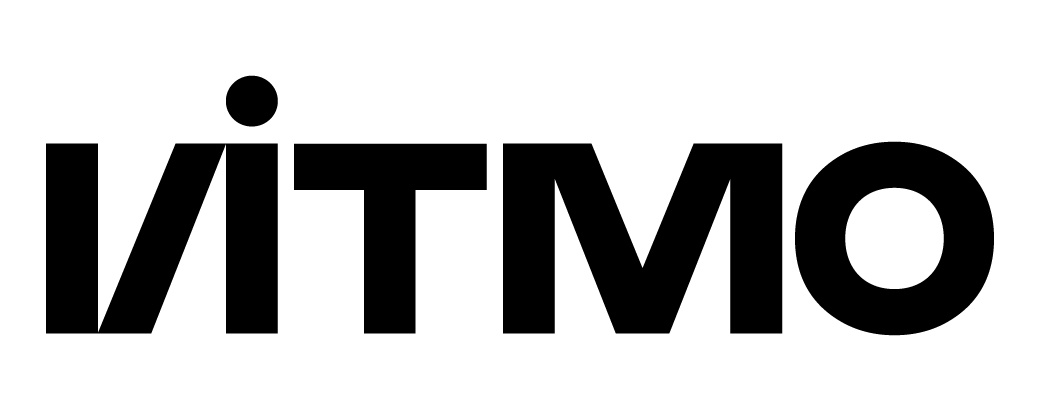
\includegraphics[width=\textwidth]{logo.png}
    % LAB INFO
    {
        \Large
        \textbf{Лабораторная работа по физике №2}
        \par
        \normalsize
        \vspace*{0.75cm}
        \textbf{Изучение скольжения тележки по наклонной плоскости}
        \par
    }
    \vfill
    % СREDITS
    \hfill\begin{minipage}{\dimexpr\textwidth-7.8cm}
        \textbf{Выполнили:}\par
        Шпак Всеволод Васильевич\par
        Степанов Арсений Алексеевич\par
        Выдра Андрей Михайлович\par
        \vspace*{0.15cm}
        \textbf{Группа:}\par
        ФИЗ ПИиКТ БАЗ 3.4.1\par 
        \vspace*{0.15cm}
        \textbf{Преподаватель:}\par
        Пулькин Николай Сергеевич\par
    \end{minipage}
    \vfill
    Санкт-Петербург, \the\year{}г.
\end{titlepage}  
\section{Цели работы}
Экспериментальная проверка равноускоренности движения тележки по наклонной плоскости и определение величины ускорения свободного падения $g$
\subsection{Задачи, решаемые при выполнении работы}
\begin{itemize}
    \item Измерение времени движения тележки по рельсу с фиксированным углом наклона
    \item Измерение времени движения тележки по рельсу при разных углах наклона рельса к горизонту
    \item Исследование движения тележки при фиксированном угле наклона рельса. Проверка равноускоренности движения тележки
    \item Исследование зависимости ускорения тележки от угла наклона рельса к горизонту. Определение ускорения свободного падения
    \item Обработка экспериментальных данных
\end{itemize}
\section{Схема установки}
\begin{center}
    \includegraphics*[width=14cm]{setup.png}
\end{center}
\begin{enumerate}
    \item Рельс с сантиметровой шкалой на лицевой стороне
    \item Тележка
    \item Воздушный насос
    \item Источник питания насоса
    \item Опоры рельса
    \item Опорная плоскость (поверхность стола)
    \item Фиксирующий электромагнит
    \item Оптические ворота
    \item Цифровой измерительный прибор ПКЦ-3
    \item Пульт дистанционного управления прибором ПКЦ-3
    \item Линейка–угольник 
\end{enumerate}
\subsection{Измерительные приборы}
\begin{tabular}{|c|c|c|c|c|}
    \hline
    № & Наименование & Тип & Используемый диапазон & Погрешность \\
    \hline
    1 & Линейка на рельсе & - & 0 - 1.3 м & $\pm 5$ мм \\
    \hline
    2 & Линейка на угольнике & - & 0 - 25 см & $\pm 0.5$ мм \\
    \hline
    3 & Секундомер (ПКЦ-3) & Электронный & 0 - 100 с & $\pm 0.1$ с \\
    \hline
\end{tabular}
\section{Результаты прямых измерений}
\subsection{Данные рельса в горизонте}
\begin{tabular}{|c|c|c|c|}
    \hline
    $x$, мм & $x'$, мм & $h$, мм & $h'$, мм \\
    \hline
    220 & 1000 & 202 & 204 \\
    \hline
\end{tabular}
\subsection{Данные экспериментов}
\subsubsection*{Серия экспериментов №1}
\begin{tabular}{|c|c|c|c|c|c|c|}
    \hline
    № & $x_1$, м & $x_2$, м & $t_1$, с & $t_2$, с & $x_2 - x_1$, м & $(t_2^2-t_1^2) / 2$, с$^2$ \\
    \hline
    1 & 0.15 & 0.40 & 1.50 & 2.80 & 0.25 & 2.795 \\
    \hline
    2 & 0.15 & 0.50 & 1.60 & 3.30 & 0.35 & 4.165 \\
    \hline
    3 & 0.15 & 0.70 & 1.50 & 3.80 & 0.55 & 6.095 \\
    \hline
    4 & 0.15 & 0.90 & 1.60 & 4.40 & 0.75 & 8.4   \\
    \hline
    5 & 0.15 & 1.10 & 1.70 & 4.90 & 0.95 & 10.56 \\
    \hline
\end{tabular}
\subsubsection*{Серия экспериментов №2.1}
\begin{tabular}{|c|c|c|c|c|}
    \hline
    № & \multicolumn{1}{l|}{$h$, м} & \multicolumn{1}{l|}{$h'$, м} & $t_1$, с & $t_2$, с \\
    \hline
    1 & \multirow{5}{*}{210}        & \multirow{5}{*}{204}         & 1.6      & 4.9      \\
    \cline{1-1} \cline{4-5} 
    2 &                             &                              & 1.5      & 4.8      \\
    \cline{1-1} \cline{4-5} 
    3 &                             &                              & 1.6      & 4.8      \\
    \cline{1-1} \cline{4-5} 
    4 &                             &                              & 1.4      & 4.7      \\
    \cline{1-1} \cline{4-5} 
    5 &                             &                              & 1.5      & 4.7      \\
    \hline
\end{tabular}
\subsubsection*{Серия экспериментов №2.2}
\begin{tabular}{|c|c|c|c|c|}
    \hline
    № & $h$, м               & $h'$, м              & $t_1$, с & $t_2$, с \\
    \hline
    1 & \multirow{5}{*}{220} & \multirow{5}{*}{204} & 1.0      & 3.3      \\
    \cline{1-1} \cline{4-5} 
    2 &                      &                      & 1.0      & 3.2      \\
    \cline{1-1} \cline{4-5} 
    3 &                      &                      & 1.0      & 3.3      \\
    \cline{1-1} \cline{4-5} 
    4 &                      &                      & 1.0      & 3.3      \\
    \cline{1-1} \cline{4-5} 
    5 &                      &                      & 1.0      & 3.2      \\
    \hline
\end{tabular}
\subsubsection*{Серия экспериментов №2.3}
\begin{tabular}{|c|c|c|c|c|}
    \hline
    № & $h$, м               & $h'$, м              & $t_1$, с & $t_2$, с \\
    \hline
    1 & \multirow{5}{*}{230} & \multirow{5}{*}{204} & 0.8      & 2.7      \\
    \cline{1-1} \cline{4-5} 
    2 &                      &                      & 0.8      & 2.6      \\
    \cline{1-1} \cline{4-5} 
    3 &                      &                      & 0.8      & 2.6      \\
    \cline{1-1} \cline{4-5} 
    4 &                      &                      & 0.8      & 2.6      \\
    \cline{1-1} \cline{4-5} 
    5 &                      &                      & 0.8      & 2.6      \\
    \hline
\end{tabular}
\subsubsection*{Серия экспериментов №2.4}
\begin{tabular}{|c|c|c|c|c|}
    \hline
    № & $h$, м               & $h'$, м              & $t_1$, с & $t_2$, с \\
    \hline
    1 & \multirow{5}{*}{239} & \multirow{5}{*}{205} & 0.7      & 2.2      \\
    \cline{1-1} \cline{4-5} 
    2 &                      &                      & 0.7      & 2.3      \\
    \cline{1-1} \cline{4-5} 
    3 &                      &                      & 0.6      & 2.2      \\
    \cline{1-1} \cline{4-5} 
    4 &                      &                      & 0.7      & 2.3      \\
    \cline{1-1} \cline{4-5} 
    5 &                      &                      & 0.7      & 2.3      \\
    \hline
\end{tabular}
\subsubsection*{Серия экспериментов №2.5}
\begin{tabular}{|c|c|c|c|c|}
    \hline
    № & $h$, м               & $h'$, м              & $t_1$, с & $t_2$, с \\
    \hline
    1 & \multirow{5}{*}{249} & \multirow{5}{*}{205} & 0.6      & 2.0      \\
    \cline{1-1} \cline{4-5} 
    2 &                      &                      & 0.6      & 2.0      \\
    \cline{1-1} \cline{4-5} 
    3 &                      &                      & 0.6      & 2.0      \\
    \cline{1-1} \cline{4-5} 
    4 &                      &                      & 0.6      & 2.0      \\
    \cline{1-1} \cline{4-5} 
    5 &                      &                      & 0.6      & 2.0      \\
    \hline
\end{tabular}
\section{Результаты косвенных измерений}
\subsection{Используемые формулы}
\subsubsection{Выборочное значение}
$$\langle t\rangle_N=\frac{1}{N}\cdot \sum_{i=1}^Nt_i$$
\subsubsection{Среднеквадратичное отклонение среднего значения}
$$\sigma_{\langle t\rangle}=\sqrt{\frac{1}{N(N-1)}\cdot\sum_{i=1}^N(t_i - \langle t\rangle_N)^2}$$
\subsubsection{Доверительный интервал случайной погрешности}
$$\Delta_t=t_{\alpha n}\cdot\sigma_{\langle t\rangle}\qquad\alpha=0.95$$
\subsubsection{Расчёт погрешности для ускорения}
$$\Delta a = \langle a \rangle\cdot\sqrt{\frac{(\Delta x_2)^2 + (\Delta x_1)^2}{(x_2 - x_1)^2} + 4 \cdot \frac{(\langle t_1 \rangle\Delta t_1)^2 + (\langle t_2 \rangle\Delta t_2)^2}{(\langle t_2 \rangle^2 - \langle t_1 \rangle^2)^2}}$$
\subsubsection{Расчёт ускорения}
$$B=\frac{\sum^N_{i=1}{a_i\cdot\sin\alpha_i}-\frac{1}{N}\sum^N_{i=1}{a_i}\sum^N_{i=1}\sin\alpha_i}{\sum^N_{i=1}\sin\alpha_i^2-\frac{1}{N}(\sum^N_{i=1}{\sin \alpha_i})^2}$$
$$A=\frac{1}{n}(\sum^N_{i=1}a_i-B\cdot\sum^N_{i=1}\sin\alpha_i)$$
\subsection{Расчёт вспомогательных величин}
\begin{tabular}{|c|c|c|c|c|c|}
    \hline
    & серия 2.1 & серия 2.2 & серия 2.3 & серия 2.4 & серия 2.5 \\
    \hline
    $\langle t_1 \rangle$ & 1.520 & 1.000 & 0.800 & 0.680 & 0.600 \\
    \hline
    $\langle t_2 \rangle$ & 4.780 & 3.260 & 2.620 & 2.260 & 2.000 \\
    \hline
    $\Delta_{t_1}$ & 0.045 & 0.000 & 0.000 & 0.024 & 0.000 \\
    \hline
    $\Delta t_1$ & 0.067 & 0.050 & 0.050 & 0.055 & 0.050 \\
    \hline
    $\Delta_{t_2}$ & 0.045 & 0.029 & 0.024 & 0.029 & 0.000 \\
    \hline
    $\Delta t_2$ & 0.067 & 0.058 & 0.055 & 0.058 & 0.050 \\
    \hline
    $\langle a \rangle$ & 0.093 & 0.197 & 0.305 & 0.409 & 0.522 \\
    \hline
    $\Delta a$ & 0.003 & 0.008 & 0.015 & 0.024 & 0.030 \\
    \hline
\end{tabular}
\subsection{Расчёт ускорения и погрешностей}
\begin{tabular}{|c|c|c|c|c|}
    \hline
    Кол-во пластин & $\sin\alpha$ & $t_1$, с & $t_2$, с & $a$, м/с$^2$ \\
    \hline
    1 & 0.010256410 & $1.520 \pm 0.067$ & $4.780 \pm 0.067$ & $0.093 \pm 0.003$ \\
    \hline
    2 & 0.023076923 & $1.000 \pm 0.050$ & $3.260 \pm 0.058$ & $0.197 \pm 0.008$ \\
    \hline
    3 & 0.035897436 & $0.800 \pm 0.050$ & $2.620 \pm 0.055$ & $0.305 \pm 0.015$ \\
    \hline
    4 & 0.046153846 & $0.680 \pm 0.055$ & $2.260 \pm 0.058$ & $0.409 \pm 0.024$ \\
    \hline
    5 & 0.058974359 & $0.600 \pm 0.050$ & $2.000 \pm 0.050$ & $0.522 \pm 0.030$ \\
    \hline
\end{tabular}
\section{Графики}
\subsection{Зависимость $Y=aZ$}
\begin{center}
    \includegraphics*[width=14cm]{graph_1.png}
\end{center}
\subsection{Зависимость $a=A+B\cdot\sin\alpha$}
\begin{center}
    \includegraphics*[width=14cm]{graph_2.png}
\end{center}
\section{Окончательные результаты}
$$B=g=8.873 \qquad A=-0.004$$
$$\delta_g=\sqrt{\frac{\sum^N_{i=1}d_i^2}{D(N-2)}}\qquad d_i=a_i - (A + B\cdot\sin\alpha_i)\qquad D=\sum^N_{i=1}\sin\alpha_i^2-\frac{1}{N}(\sum^N_{i=1}{\sin \alpha_i})^2$$
$$D=0.001454\qquad\delta_g=0.490\qquad\Delta g = 2\cdot\delta_g = 0.98$$
$$\epsilon=\frac{\Delta g}{g}\cdot 100\%=11\%$$
\section{Выводы}
В первой части задания была доказана линейная зависимость $Y(Z)=a\cdot Z$, где $Y$ – перемещение тележки по рельсу, когда мы измеряли время, а $Z$ – квадрат времени, за которое было произведено это перемещение. Следовательно, движение равноускоренное. \\
\hfill\break
Во второй части работы, проанализировав скорость движения тележки и её ускорение мы смогли определить значение ускорения свободного падения: $g=8.873\pm0.98$ м/c$^2$ с относительной погрешностью в 11\% \\
\end{document}
